\documentclass[10pt,a4paper]{article}
\usepackage[utf8]{inputenc}
\usepackage{amsmath}
\usepackage{amsfonts}
\usepackage{amssymb}
\usepackage{graphicx}
\title{The Riddler Solution}
\date{June 3rd 2022}
\author{Eric Dallal}
\DeclareMathOperator*{\argmin}{arg\,min}
\begin{document}
\maketitle
\textbf{Problem Statement}:\\

From Jason Zimba comes a surprisingly sandy puzzle:\\

In the Great Riddlerian Desert, there is a single oasis that is straight and narrow. There are N travelers who are trapped at the oasis, and one day, they agree that they will all leave. They independently pick a random location in the oasis from which to start and a random direction in which to travel. Once their supplies are packed, they all head out.\\

What is the probability that none of their paths will intersect, in terms of N? (For the purposes of this puzzle, assume the oasis is a line segment, while the desert is an infinite Cartesian plane.)\\

\textbf{Solution}:\\

Suppose that the desert is a line segment on the $x$ axis. Then the $N$ travelers can be split into two groups: those that depart in the positive $y$ direction (group A) and those that depart in the negative $y$ direction (group B). Clearly, paths can only intersect for a pair of travelers within the same group.\\

Suppose that there are $k$ travelers in group A and $N-k$ travelers in group B. The paths of the group A travelers will be non-intersecting if and only if the angles that their departure directions make with the positive $x$ axis are increasing when ordering the travelers from right to left (see diagram). The probability of this happening by chance is $1/k!$. Similarly, the probability that the paths of the group B travelers are non-intersecting will be $1/(N-k)!$.\\

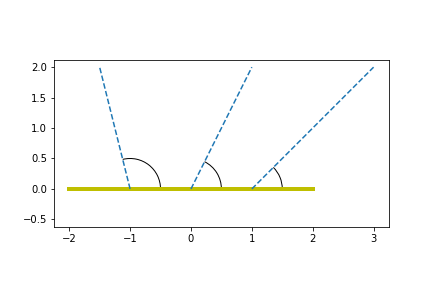
\includegraphics[width=\textwidth]{Angles}

As there are ${N \choose k}$ ways to split the travelers with $k$ in group A and $N-k$ in group B, and there are $2^N$ equally likely partitions of the $N$ travelers into the two groups, it follows that the probability that all their paths will be non-intersecting is:

\begin{equation}
P(N) := \frac{1}{2^N}\sum_{k = 0}^{N}{N \choose k}\frac{1}{k!}\frac{1}{(N-k)!}
\end{equation}

This equation can be simplified thanks to a combinatorial identity and some math:

\begin{eqnarray*}
P(N) & = & \frac{1}{2^N}\sum_{k = 0}^{N}{N \choose k}\frac{1}{k!}\frac{1}{(N-k)!}\\
 & = & \frac{1}{N!2^N}\sum_{k = 0}^{N}{N \choose k}^2\\
 & = & \frac{1}{N!2^N}{2N \choose N}\\
 & = & \frac{(2N)!}{(N!)^3 2^N}\\
 & = & \frac{(2N-1)!!}{(N!)^2}
\end{eqnarray*}
where $(2N-1)!! = 1\cdot 3\cdot \ldots \cdot (2N-1)$. See below for a plot of this function.

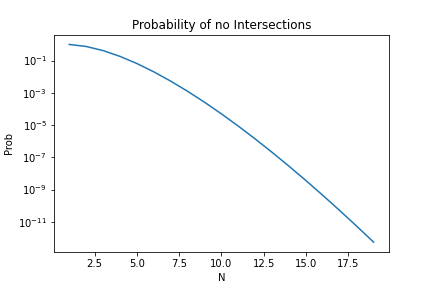
\includegraphics[width=\textwidth]{Prob}

Notably, $P(N)$ diminishes quite rapidly as a function of $N$. In fact, $P(N)/P(N-1) = (2N-1)/N^2$ so that, for large $N$, the ratio of consecutive function values is approximately $2/N$.

\end{document}